% \begin{frame}{Protein kinase interaction inference on yeast data}
% \label{sec:yeast_results}
% \begin{columns}
% \newcommand\histwidth{0.36\textwidth}
% \begin{column}{0.5\textwidth}
% % The TF$\rightarrow$gene edges from the data are assumed to be the full set of transcription factors and the signs of their interactions are also enforced for edges where it is known in the Yeastract dataset, as described in~\autoref{sec:data_preprocess}. The inference is performed on edges with protein kinases as source node. For TFs, the model predicts edge strengths, and, in cases with unknown sign, it predicts the sign of interaction.


% \begin{figure}[ht]
% \centering
% \begin{subfigure}[b]{\histwidth}\centering\caption{}
% \includegraphics[width=\textwidth]{analysis/fig/hist_pk-tf_high_single.pdf}\label{fig:yeast_hist_single.a}
% \end{subfigure}
% \quad
% \begin{subfigure}[b]{\histwidth}\centering\caption{}
% \includegraphics[width=\textwidth]{analysis/fig/hist_pk-pk_high_single.pdf}\label{fig:yeast_hist_single.b}
% \end{subfigure}
% % \vskip\baselineskip
% \begin{subfigure}[b]{\histwidth}\centering\caption{}
% \includegraphics[width=\textwidth]{analysis/fig/hist_pk-tf_single.pdf}\label{fig:yeast_hist_single.c}
% \end{subfigure}
% \quad
% \begin{subfigure}[b]{\histwidth}\centering\caption{}
% \includegraphics[width=\textwidth]{analysis/fig/hist_pk-pk_single.pdf}\label{fig:yeast_hist_single.d}
% \end{subfigure}
% \caption{\textbf{PK edge inference on yeast.} High quality edges~(a,b) and unknown/less likely edges~(c,d). }
% \label{fig:yeast_hist_single}
% \end{figure}

% % Edge inference was attempted on the RNA log fold-change data~(\autoref{sec:yeast_data}). Densities of scores for edges from different datasets can be seen in~\autoref{fig:yeast_hist_single} for a single attempt at minimizing~$\boldsymbol{e}$ where the score is the absolute weight value, and in~\autoref{fig:yeast_hist_avgstd} normalized scores where multiple individual attempts at minimizing~$\boldsymbol{e}$ were performed and normalized so that the scores are average weight values divided by the empirical standard deviation observed for each. The LLC method was used for comparison which can be found in~\autoref{fig:yeast_hist_llc} in the appendix, where it can be seen that there is no clear difference between datasets. Inference was also attempted by letting the score of an edge be the average weight from multiple individual minimization of~$\boldsymbol{e}$, with similar results to the normalized attempt~(\autoref{fig:yeast_hist_avg}). All density plots are split into subplots for datasets where we expect all edges should be true edges and the low confidence datasets biogrid and the category "unknown" which holds all entries of the adjacency matrix where an edge is possible, yet not found in any of the other datasets.

% \end{column}
% \begin{column}{0.5\textwidth}
% \begin{figure}[ht]
% \centering
% \begin{subfigure}[b]{\histwidth}\centering\caption{}
% \includegraphics[width=\textwidth]{analysis/fig/hist_pk-tf_high_avgstd.pdf}
% \end{subfigure}
% \quad
% \begin{subfigure}[b]{\histwidth}\centering\caption{}
% \includegraphics[width=\textwidth]{analysis/fig/hist_pk-pk_high_avgstd.pdf}
% \end{subfigure}
% % \vskip\baselineskip
% \begin{subfigure}[b]{\histwidth}\centering\caption{}
% \includegraphics[width=\textwidth]{analysis/fig/hist_pk-tf_avgstd.pdf}
% \end{subfigure}
% \quad
% \begin{subfigure}[b]{\histwidth}\centering\caption{}
% \includegraphics[width=\textwidth]{analysis/fig/hist_pk-pk_avgstd.pdf}
% \end{subfigure}
% \caption{\textbf{Normalized PK edge inference on yeast.} High quality edges~(a,b) and unknown/less likely edges~(c,d). }
% \label{fig:yeast_hist_avgstd}
% \end{figure}
% \end{column}
% % We observe that two peaks appear in the density plots, at around score=\num{1e-4} and score=\num{3e-2} for~\autoref{fig:yeast_hist_single} as well as score=\num{1e-1} and score=\num{1e+1} for~\autoref{fig:yeast_hist_avgstd}. The peaks are visible for PK$\rightarrow$TF edges but PK$\rightarrow$PK edge inference is not clearly divided. The peaks can be useful for categorizing edges as present or absent, with the peak at lower score classifying absence of edges and the other indicating presence. We see that for datasets with edges assumed to be known, there are higher densities for peaks at higher scores~(\autoref{fig:yeast_hist_single.a}). This is especially seen for Fasolo~et~al. data but barely for EMAP data~\autoref{sec:fiedler_data}. The opposite is the case for datasets where the edge presence and absence are unknown~(\autoref{fig:yeast_hist_single.c}). Since the adjacency matrices should overall be sparse there would be many non-edges. 
% \end{columns}
% \end{frame}

\begin{frame}{Inference performance}
\begin{columns}
\begin{column}{0.2\textwidth}
(A) Simulated data \\
(B-C) Yeast data
\begin{itemize}
    \item No negative examples
    \item Few datapoints
\end{itemize}
\end{column}

\begin{column}{0.8\textwidth}
\begin{figure}[ht]
    \centering
    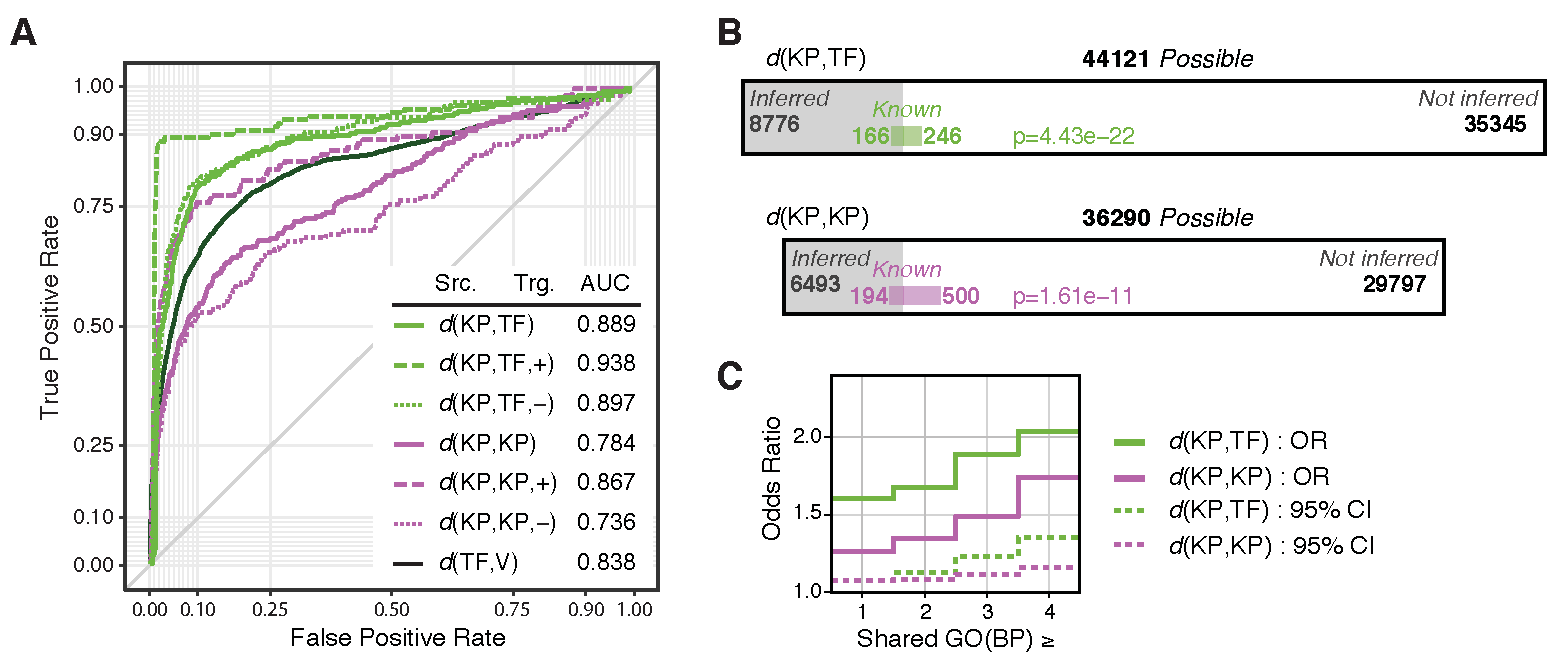
\includegraphics[width=0.85\textwidth]{analysis/fig/Fig3.pdf}
    \caption{\textbf{Performance on simulated and yeast data.} \\  }
    \label{fig:minimum_performance}
\end{figure}
% Since the datasets for evaluation of performance only provides examples of presence of edges~(positive examples), we cannot directly evaluate balance between accuracy, specificity, etc. for the model. By using all possible edges not in a dataset of known edges we get a minimum performance where many of the datapoints used as negatives are in fact positives~(\autoref{fig:minimum_performance}). The Fiedler dataset with PK$\rightarrow$TF edges is included, since it was the single dataset with best performance. We see that PK$\rightarrow$PK edges from any dataset has no noticeably higher scoring than edges not in the dataset. PK$\rightarrow$TF edges from the datasets with known edges has a clear but small overrepresentation as larger scoring edges compared to other possible edges.
\end{column}
\end{columns}
\end{frame}
